%!TEX root = ../../../thesis.tex

This chapter begins with a mathematical analysis of streaming cells and operating parameters.
Then, in \cref{sect:part1_energyHarvesting_buildingStreamingCells}, a variety of streaming cell designs are built.
Early attempts at making streaming cells are presented, followed by more successful streaming cell designs.
Ten streaming cells are made using that design with each having slightly different geometric dimensions.
The electrical output and energy conversion efficiency of these cells is measured in \cref{sect:part1_energyHarvesting_measuringStreamingCells}.
Measurement results are discussed in~\cref{sect:part1_energyHarvesting_discussion}, followed by my concluding remarks.


\section{General Analysis}
  \label{sect:part1_energyHarvesting_generalAnalysis}


  A basic model of operation for a streaming cell is established.
  This determines what parameters are important when maximising a cell's output power.


  \subsection{Mathematics}


    Mathematical analysis of streaming cells provides a basic understanding of the parameters involved with their output and geometry.
    Rigorous mathematical analysis of streaming cell performance is extremely involved and is well detailed in the literature~\cite{Yang1998}.
    As aspects of a double layer's structure are still not fully understood, the mathematics behind them is still being developed.
    Computer simulation and mathematical models continue to shed light on ionic organisation at liquid-solid interfaces~\cite{Kornyshev2007}.
    For that reason, I have not attempted to model a streaming cell physically.
    Instead, I piece together a relatively simple mathematical model quantifying important operating parameters.


    \subsubsection*{Streaming voltage}

      Gu and Li derived the following equation relating the streaming voltage to the pressure applied across a streaming cell~\cite{Gu2000}.
      \begin{equation}
      \frac{V_{s}}{\Delta P} = \frac{\varepsilon_{r}\,\varepsilon_{0}\,\zeta}{\mu(\sigma+\frac{2}{\delta}\lambda)}
      \label{eq:part1_energyHarvesting_streamingVoltage}
      \end{equation}
      \noindent where:
      \begin{description}
          \item $V_{s}$ is streaming voltage,
          \item $\Delta P_{z}$ is pressure differential (across the channel),
          \item $\epsilon_{r}$ is the relative permittivity of the liquid,
          \item $\epsilon_{0}$ is the absolute permittivity of free space,
          \item $\zeta$ is zeta potential,
          \item $\mu$ is the fluid's viscosity,
          \item $\sigma$ is the fluid's bulk conductivity,
          \item $\delta$ is the channel's height (refer to \cref{fig:width_height_length}),
          \item $\lambda$ is the channel's surface conductivity.
      \end{description}
      This equation is specific to parallel plate channels, of the type constructed in the following section.
      It requires that the width of the channel's cross-section is a minimum of twenty times larger than its height, which it is for the cells constructed here.
      Gu and Li use this equation as a means of finding the zeta potential and surface conductance by rearranging it into the following form:
      \begin{equation}
        \frac{\varepsilon_{r}\, \varepsilon_{0}\, \Delta P}{\mu\, V_{s}\, \sigma} = \frac{1}{\zeta} + \left(\frac{2\, \lambda}{\zeta\, \sigma}\right)\, \frac{1}{\delta}
      \end{equation}
      Later, the streaming voltage of ten cells with the same dimensions of those used by Gu and Li will be measured.
      The left hand side of this equation will be plotted against the inverse of channel height to see if their results can be replicated.
      If successful, this will give a way of determining the zeta potential and surface conductance of the fabricated cells.


    \subsubsection*{Streaming current}


      Gu and Li, also derive a similar equation for streaming current~\cite{Gu2000}.
      This equation, shown below, has been slightly rearranged to match the form of~\cref{eq:part1_energyHarvesting_streamingVoltage}
      \begin{equation}
          \frac{I_{s}}{\Delta P} = \frac{\varepsilon_{r}\,\varepsilon_{0}\,\zeta\,W\,\delta}{\mu\,L}
          \label{eq:part1_energyHarvesting_streamingCurrent}
      \end{equation}
      where:
      \begin{description}
          \item $W$ is the width of the channel,
          \item $L$ is the length of the channel.
      \end{description}
      This equation is similar to that given by Olthuis et al.\ for a porous plug, but has been derived specifically for rectangular channels\cite{Olthuis2005}.


  \subsection{Electrical model}
    \label{sub:part1_energyHarvesting_generalAnalysis_electricalModel}


    % Model
    \begin{figure}
        \centering
            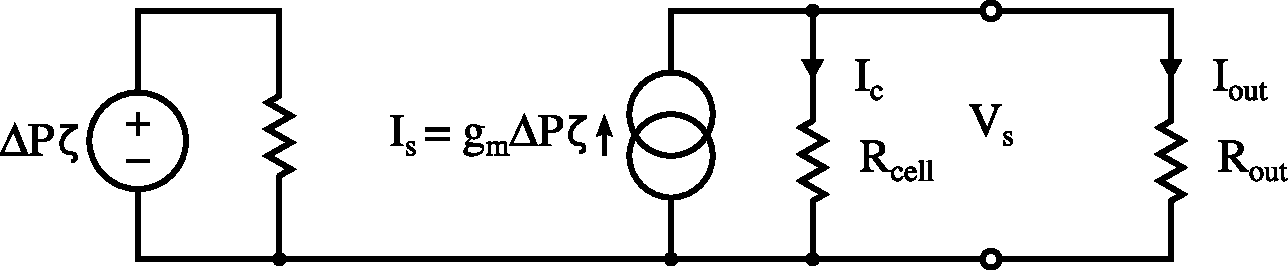
\includegraphics[width=\textwidth]{content/pt1/01-PowerHarvesting/graphics/StreamingCell_EquivalentCircuit_output}
        \caption{\label{fig:StreamingCell_Schematic-representation}Schematic diagram of a streaming cell with connected load resistance.}
    \end{figure}
    Figure \ref{fig:StreamingCell_Schematic-representation} depicts schematically how a streaming cell operates when connected to an external load.
    A model of this sort is commonly used to analyse the behaviour transistors.
    This particular model is based on the work of Olthuis et al.\ in \cite{Olthuis2005}, but has been modified slightly.
    Instead of showing the zeta potential ($\zeta$) as the equivalent voltage source, it is shown here instead with the pressure applied ($\Delta P$).
    This change was made because there is no way of controlling the zeta potential - it determined by the properties of the particular interface.
    However, the amount of pressure developed across the cell is controllable, and from \cref{eq:part1_energyHarvesting_streamingCurrent} it is shown to be directly proportional to streaming current.
    In fact, the transconductance ($g_{m}$) for this model is \cref{eq:part1_energyHarvesting_streamingCurrent}.
    The model aids analysis in that it shows the electrical configuration of an external load resistance ($R_{out}$).
    As shown, any load resistance placed across the cell is being placed in parallel with the internal electrical resistance of the cell.
    This will help to determine how best to optimise the cell in order to maximise its electrical output.


  \subsection{Optimisation}

    Having a mathematical model of a streaming cell allows for optimisation of its operating parameters.
    The model shows that any load placed across a streaming cell is actually placed in parallel with that cell's internal resistance.
    Therefore, choosing a suitable load is an important design consideration.
    It is possible to optimise the cell's output for maximum power output, or maximum efficiency.
    So which is best suited to harvesting applications?
    The only time energy can be extracted from a streaming cell is when pressure developed across it because of liquid flowing through it.
    When power is available to harvest, it is beneficial to collect as much as possible -- no matter how much is wasted.
    Any energy that we could not capture will be lost.
    In situations requiring maximum efficiency, the efficiency of the system approaches \SI{100}{\percent} as the power delivered approaches \SI{0}{\percent}.
    In situations requiring maximum power, the maximum achievable efficiency is \SI{50}{\percent}.
    This means we can only harness half of the electrical power developed by a cell, at best.


    % Contrasting this view, consider battery powered applications.
    % In those situations often optimise power usage for maximum efficiency.
    % Doing so conserves energy in the battery and ensures as little as possible goes to waste.


    \subsubsection*{Optimising $R_{out}$ for maximum power}


      Using Ohm's Law it is possible to form an equation linking the total power ($P_{cell}$) to the total electrical resistance across the cell ($R_{tot}$).
      \begin{align}
          P & = V\times I\nonumber \\
          V & = I\times R\nonumber \\
          P & = I^{2}\times R\nonumber \\
          P_{cell} & = I_{s}^{2}\times R_{tot}
          \label{eq:DeterminingOutputPower_basic}
      \end{align}
      Where $I_{s}$ is the streaming current created by pumping ions through the channel.
      As the output resistance and internal cell resistance are in parallel we can find the output current ($I_{out}$) by treating the cell as a resistor divider (as is shown in~\cref{fig:StreamingCell_Schematic-representation}).
      Using a resistor divider equation for current in parallel branches yields:
      \begin{align}
          I_{out} & = I_{s}\times\frac{R_{cell}}{R_{cell}+R_{out}}
          \label{eq:DeterminingOutputPower_extended}
      \end{align}
      Combining \cref{eq:DeterminingOutputPower_basic} and \cref{eq:DeterminingOutputPower_extended} we can extract the power dissipated in a load attached across the cell.
      \begin{align}
          I_{out} & = I_{s}\times\frac{R_{cell}}{R_{cell}+R_{out}}\nonumber \\
          P_{out} & = \left[I_{s}\times\frac{R_{cell}}{R_{cell}+R_{out}}\right]^{2}\times R_{out}
          \label{eq:DeterminingOutputPower_result}
      \end{align}

      \Cref{eq:DeterminingOutputPower_result} takes into account the internal dissipation within the cell due to its own internal resistance.
      In order to optimise the output power it is necessary to find the value of output resistance ($R_{out}$) that maximises the output power.

      A parallel resistance system where we try to maximise the output power suggests this is a maximum power transfer theorem problem.
      The maximum power transfer theorem states that in order to maximise the power delivered to an external load from a source which itself has an internal resistance, one must make the two resistance equal.


    % \subsubsection*{Maximum power transfer theorem for a current source}


    %   This theorem is shown for resistors in series but no clear proof was found for a current source with two resistances in parallel.
    %   Here I prove that the maximum power theorem holds for a current source with resistors in parallel.
    %   This is not new work, but is included for completeness.

    %   First we take \cref{eq:DeterminingOutputPower_result} and treat the streaming current ($I_{s}$) as a constant, differentiate with respect to $R_{out}$ and find the condition that gives a maximum/minimum power output.
    %   \begin{eqnarray}
    %       P_{out} & = & \left[I_{s}\times\frac{R_{cell}}{R_{cell}+R_{out}}\right]^{2}\times R_{out}\nonumber\\
    %       \frac{P_{out}}{R_{out}} & = & \left[1\times\frac{R_{cell}}{R_{cell}+R_{out}}\right]^{2}\nonumber\\
    %       \frac{\partial P_{out}}{\partial R_{out}} & = & \frac{R_{cell}^{2}}{(R_{cell}+R_{out})^{2}}-\frac{2\times R_{cell}^{2}\times R_{out}}{(R_{cell}+R_{out})^{3}}\nonumber\\
    %       0 & = & \frac{R_{cell}^{2}}{(R_{cell}+R_{out})^{2}}-\frac{2\times R_{cell}^{2}\times R_{out}}{(R_{cell}+R_{out})^{3}}\nonumber\\
    %       \frac{2\times R_{cell}^{2}\times R_{out}}{(R_{cell}+R_{out})^{3}} & = & \frac{R_{cell}^{2}}{(R_{cell}+R_{out})^{2}}\nonumber\\
    %       \frac{2\times R_{cell}^{2}\times R_{out}}{R_{cell}+R_{out}} & = & R_{cell}^{2}\nonumber\\
    %       2\times R_{cell}^{2}\times R_{out} & = & R_{cell}^{2}\times(R_{cell}+R_{out})\nonumber\\
    %       2\times R_{out} & = & R_{cell}+R_{out}\nonumber\\
    %       R_{out} & = & R_{cell}
    %       \label{eq:maximumPowerTheorem_norton}
    %   \end{eqnarray}

    %   This shows that there is either maximum or minimum power transfer to $R_{out}$ when the value of $R_{out}$ matches that of $R_{cell}$.
    %   By plotting the power output as a function of the ratio of the two resistances (shown in \cref{fig:Plot-of-PowerTheorem}), we can see it is indeed a maximum.
    %   This shows the assumption of the maximum power transfer theorem in the case of streaming cell output to be correct.
    %   Usefully, it is shown that the absolute magnitudes of both $R_{out}$ and $R_{cell}$ have no effect on the output power - only their relative sizes (which in this case is equal).

    %   \begin{figure}
    %       \centering
    %           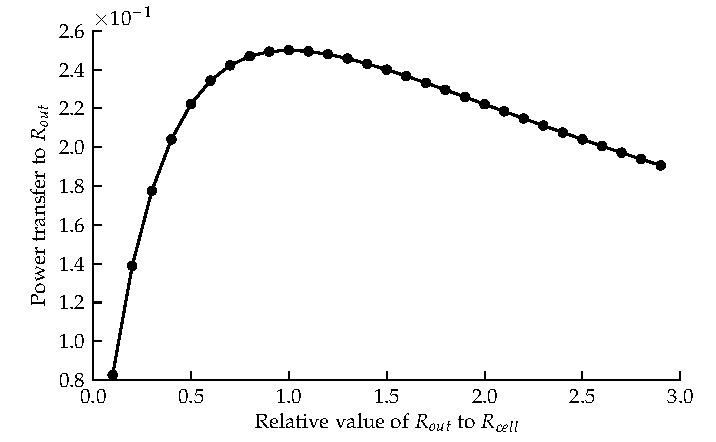
\includegraphics{content/pt1/01-PowerHarvesting/graphics/maximumPowerThereom}
    %       \caption{\label{fig:Plot-of-PowerTheorem}Plot of Equation \ref{eq:DeterminingOutputPower_result} when $I_{s}=1A$ and $R_{cell}=1\Omega$}
    %   \end{figure}


    \subsubsection*{Optimising streaming cell parameters}


      We now use the optimised values of $R_{out}$ and $R_{cell}$ to calculate the maximum available power.
      This is done by substituting $R_{out}$ and $R_{cell}$ for $R$ in \cref{eq:DeterminingOutputPower_result}:
      \begin{align}
          P_{out} & = \left[I_{s}\times\frac{R_{cell}}{R_{cell}+R_{out}}\right]^{2}\times R_{out}\nonumber \\
          P_{max} & = \left[I_{s}\times\frac{1}{2}\right]^{2}\times R\nonumber \\
          P_{max} & = \frac{I_{s}^{2}R}{2}
          \label{eq:streamingCell_maxPower}
      \end{align}
      As $P=I^{2}R$ (via the power equation and Ohm's Law) this indicates at best we can capture half of the available power.

      It is now possible to combine the equation for maximum power, \cref{eq:streamingCell_maxPower}, and that for streaming current, \cref{eq:part1_energyHarvesting_streamingCurrent}.
      \begin{align}
          P_{max} & = \frac{I_{s}^{2}R}{2}\nonumber \\
          P_{max} & = \left(\frac{\varepsilon\,\zeta\,W\,\delta\,\Delta P}{\mu\,L}\right)^{2}\times\frac{R}{2}
          \label{eq:streamingCell_maxPower_substituted}
      \end{align}
      where $\varepsilon=\varepsilon_{0}\,\varepsilon_{r}$ and $R=R_{cell}=R_{out}$.

      To get a better feel for this equation, it may help to substitute in the parameters that affect $R$.
      From here we will refer to $R$ as the internal electrical resistance of the cell.
      It also refers to the external resistance in the maximum power condition, but we are free to vary that to match the internal resistance.

      We begin with the understanding that:
      \begin{align}
          R & \propto \frac{L}{A\,\sigma}\label{eq:cell_resistance_electrical}\\
          R_{h} & \propto \frac{L\,\mu}{A}\label{eq:cell_resistance_hydro}
      \end{align}
      where $\sigma$ is the conductivity of the liquid and $A$ is the cross-sectional area of the cell.
      The first \cref{eq:cell_resistance_electrical} states that the electrical resistance will increase with cell length and decrease with the cross-sectional area of the cell and the conductivity of the fluid.
      The second \cref{eq:cell_resistance_hydro} states that the fluid mechanical resistance will increase with the length of the cell and the viscosity of the fluid, and decrease with the cross-sectional area of the cell.

      We can identify the presence of $R_{h}$ in \cref{eq:streamingCell_maxPower_substituted}.
      Starting with this equation we substitute \cref{eq:cell_resistance_electrical} in and rearrange to produce an approximate relationship between pressure, cell length and area:
      \begin{align}
          P_{max} & = \left(\frac{\varepsilon\,\zeta\,W\,\delta\,\Delta P}{\mu\,L}\right)^{2}\times\frac{R}{2}\nonumber\\
          P_{max} & \propto \left(\frac{W\,\delta}{\mu\,L}\right)^{2}\times\left(\varepsilon\,\zeta\,\Delta P\right)^{2}\times \frac{L}{A\,\sigma} \times\frac{1}{2}\nonumber\\
          P_{max} & \propto \left(\frac{A}{\mu\,L}\right)^{2}\times\left(\varepsilon\,\zeta\,\Delta P\right)^{2}\times \frac{L}{A\,\sigma} \times\frac{1}{2}\nonumber\\
          P_{max} & \propto \frac{A^{2}}{L^{2}}\times\left(\frac{\varepsilon\,\zeta\,\Delta P}{\mu}\right)^{2}\times \frac{L}{A} \times\frac{1}{2\,\sigma}\nonumber\\
          P_{max} & \propto \frac{A}{L}\times\left(\frac{\varepsilon\,\zeta\,\Delta P}{\mu}\right)^{2}\times\frac{1}{2\,\sigma}\nonumber\\
          P_{max} & \propto \left(\frac{\varepsilon\,\zeta\,\Delta P}{\mu}\right)^{2}\times\frac{A}{2\,L\,\sigma}\nonumber\\
          P_{max} & \propto \frac{\Delta P^{2}\,A}{L}\times \frac{\varepsilon^{2}\,\zeta^{2}}{2\,\mu^{2}\,\sigma}
          \label{eq:streamingCell_maxPower_relationship}
      \end{align}

      This \cref{eq:streamingCell_maxPower_relationship} suggests that a cell with a small length, large area and high pressure is the best candidate for maximising power output.
      When using tap water we have no control over the remaining parameters, highlighting the importance of cell geometry and applied pressure.


\section{Streaming Cell Fabrication}
  \label{sect:part1_energyHarvesting_buildingStreamingCells}


  Building a streaming cell seemed a simple task at the outset.
  This section gives a brief overview of the work related to creating that first working streaming cell.


  \subsection{First streaming cells}


    \begin{figure}
      \centering
      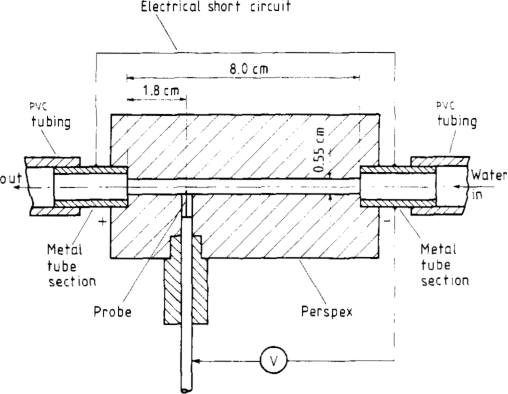
\includegraphics{content/pt1/01-PowerHarvesting/graphics/VargaSeymour1986_cell}
      \caption[Diagram of a cavitation device, taken from~\cite{Varga1986}]{\label{fig:first_cell_diagram}Diagram of a cavitation device, taken from~\cite{Varga1986}, reported to be able to generate over \SI{50}{\volt} across its ends by pumping water through it.}
    \end{figure}

    \begin{figure}
      \centering
      \includegraphics[scale=0.9]{content/pt1/01-PowerHarvesting/graphics/StreamingCell_v0}
      \caption{\label{fig:first_cell}Photo of the first streaming device built. It has been constructed form acrylic and brass by summer research student Jonathon McMullan. It was intended to create the streaming voltages reported by Varga and Seymour, but failed to produce measurable quantities of power.}
    \end{figure}
    \begin{figure}
      \centering
      \includegraphics[scale=0.7]{content/pt1/01-PowerHarvesting/graphics/StreamingCells_v1}
      \caption{\label{fig:first_cells}Photo showing two examples of a second design of streaming cell made entirely from glass.}
    \end{figure}

    The work that first sparked the interest of both my primary supervisor and I in streaming devices was that of Varga and Seymour~\cite{Varga1986}.
    In that paper it was reported that a device employing cavitation as a means of increasing the resistance between two bodies of  water was capable of developing over \SI{50}{\volt} across its ends.
    A diagram of the cavitation device is shown as \cref{fig:first_cell_diagram}.
    Summer research student Jonathon McMullan recreated that device, shown as \cref{fig:first_cell}, with the intention of reproducing results from that paper.
    The device was turned on a lathe from acrylic in two pieces and glued together.
    A brass rod (not shown) is inserted up the shaft (presented vertically in the image) into the flow of water.
    The rod had a narrow cylindrical tip, small enough to allow it to fit into the main flow pipe (presented horizontally in the image), with a flat face ground into one side.
    Water was forced through the device (left to right in the image) and the rod caused cavitation of the water as it flowed past the inserted rod tip.
    Varga and Seymour measured a potential difference of over \SI{50}{\volt} between the inserted rod and the brass end fittings using a flow rate of \SI{0.0425}{\litre\per\minute}.
    That experiment -- which tried the same flow rate, materials, liquids, and measurement setup -- did not produce measurable streaming voltage.
    % My supervisor and I became sceptical of streaming cells at this point and looked elsewhere for energy harvesting ideas.
    The following year, summer research student Wane Crump and I conducted experiments to determine the amount of charge that could be transported on water droplets.
    Research into energy harvesting with an electrostatic generator is presented in the Appendix as \cref{appendix:chargedDropletts}.

    Later, other designs of streaming cells, namely those of Gu and Li~\cite{Gu2000}, were found in the literature.
    Their design of streaming cell looked simple and easy to fabricate, so we attempted to replicate them.
    Employing Waikato University's glass-blower, Steve Newcombe, two streaming cells were fabricated entirely from soda-lime glass.
    Those streaming cells are shown in \cref{fig:first_cells}.
    Each of the two channels were made by placing a \SI{50}{\micro\meter} sheet of copper between the glass slides and then welding the slides together to seal the cell.
    The copper was etched away with acid once the cell was sealed.
    The cells were then glass welded to the side tubes that held the copper electrodes.
    By varying the length of the two channels (one of \SI{2}{\centi\meter}, the other \SI{4}{\centi\meter}) we hoped to determine what role length played on channel output characteristics.

    Both of the cells burst under the water pressure applied from lab taps.
    A crack along the right hand reservoir is visible on the \SI{2}{\centi\meter} wide channel.
    Attempts were made to strengthen the channels by coating the joins with industrial glues, but were not successful.


  \subsection{Robust streaming cells}


    The two previous attempts to create streaming cells had failed.
    In the moments before failure, the all-glass streaming cells developed measurable voltage across their terminals.
    The developed voltage was enough to warrant further pursuit, but the design needed revising in order to increase their pressure handling capability.
    A new design was found that used epoxy resin and acrylic to contain the channels.
    This design appeared to be much more resilient to cracking.
    Aspects of that design were taken from a paper by Gu and Li~\cite{Gu2000}.

    \begin{figure}[p]
      \centering
      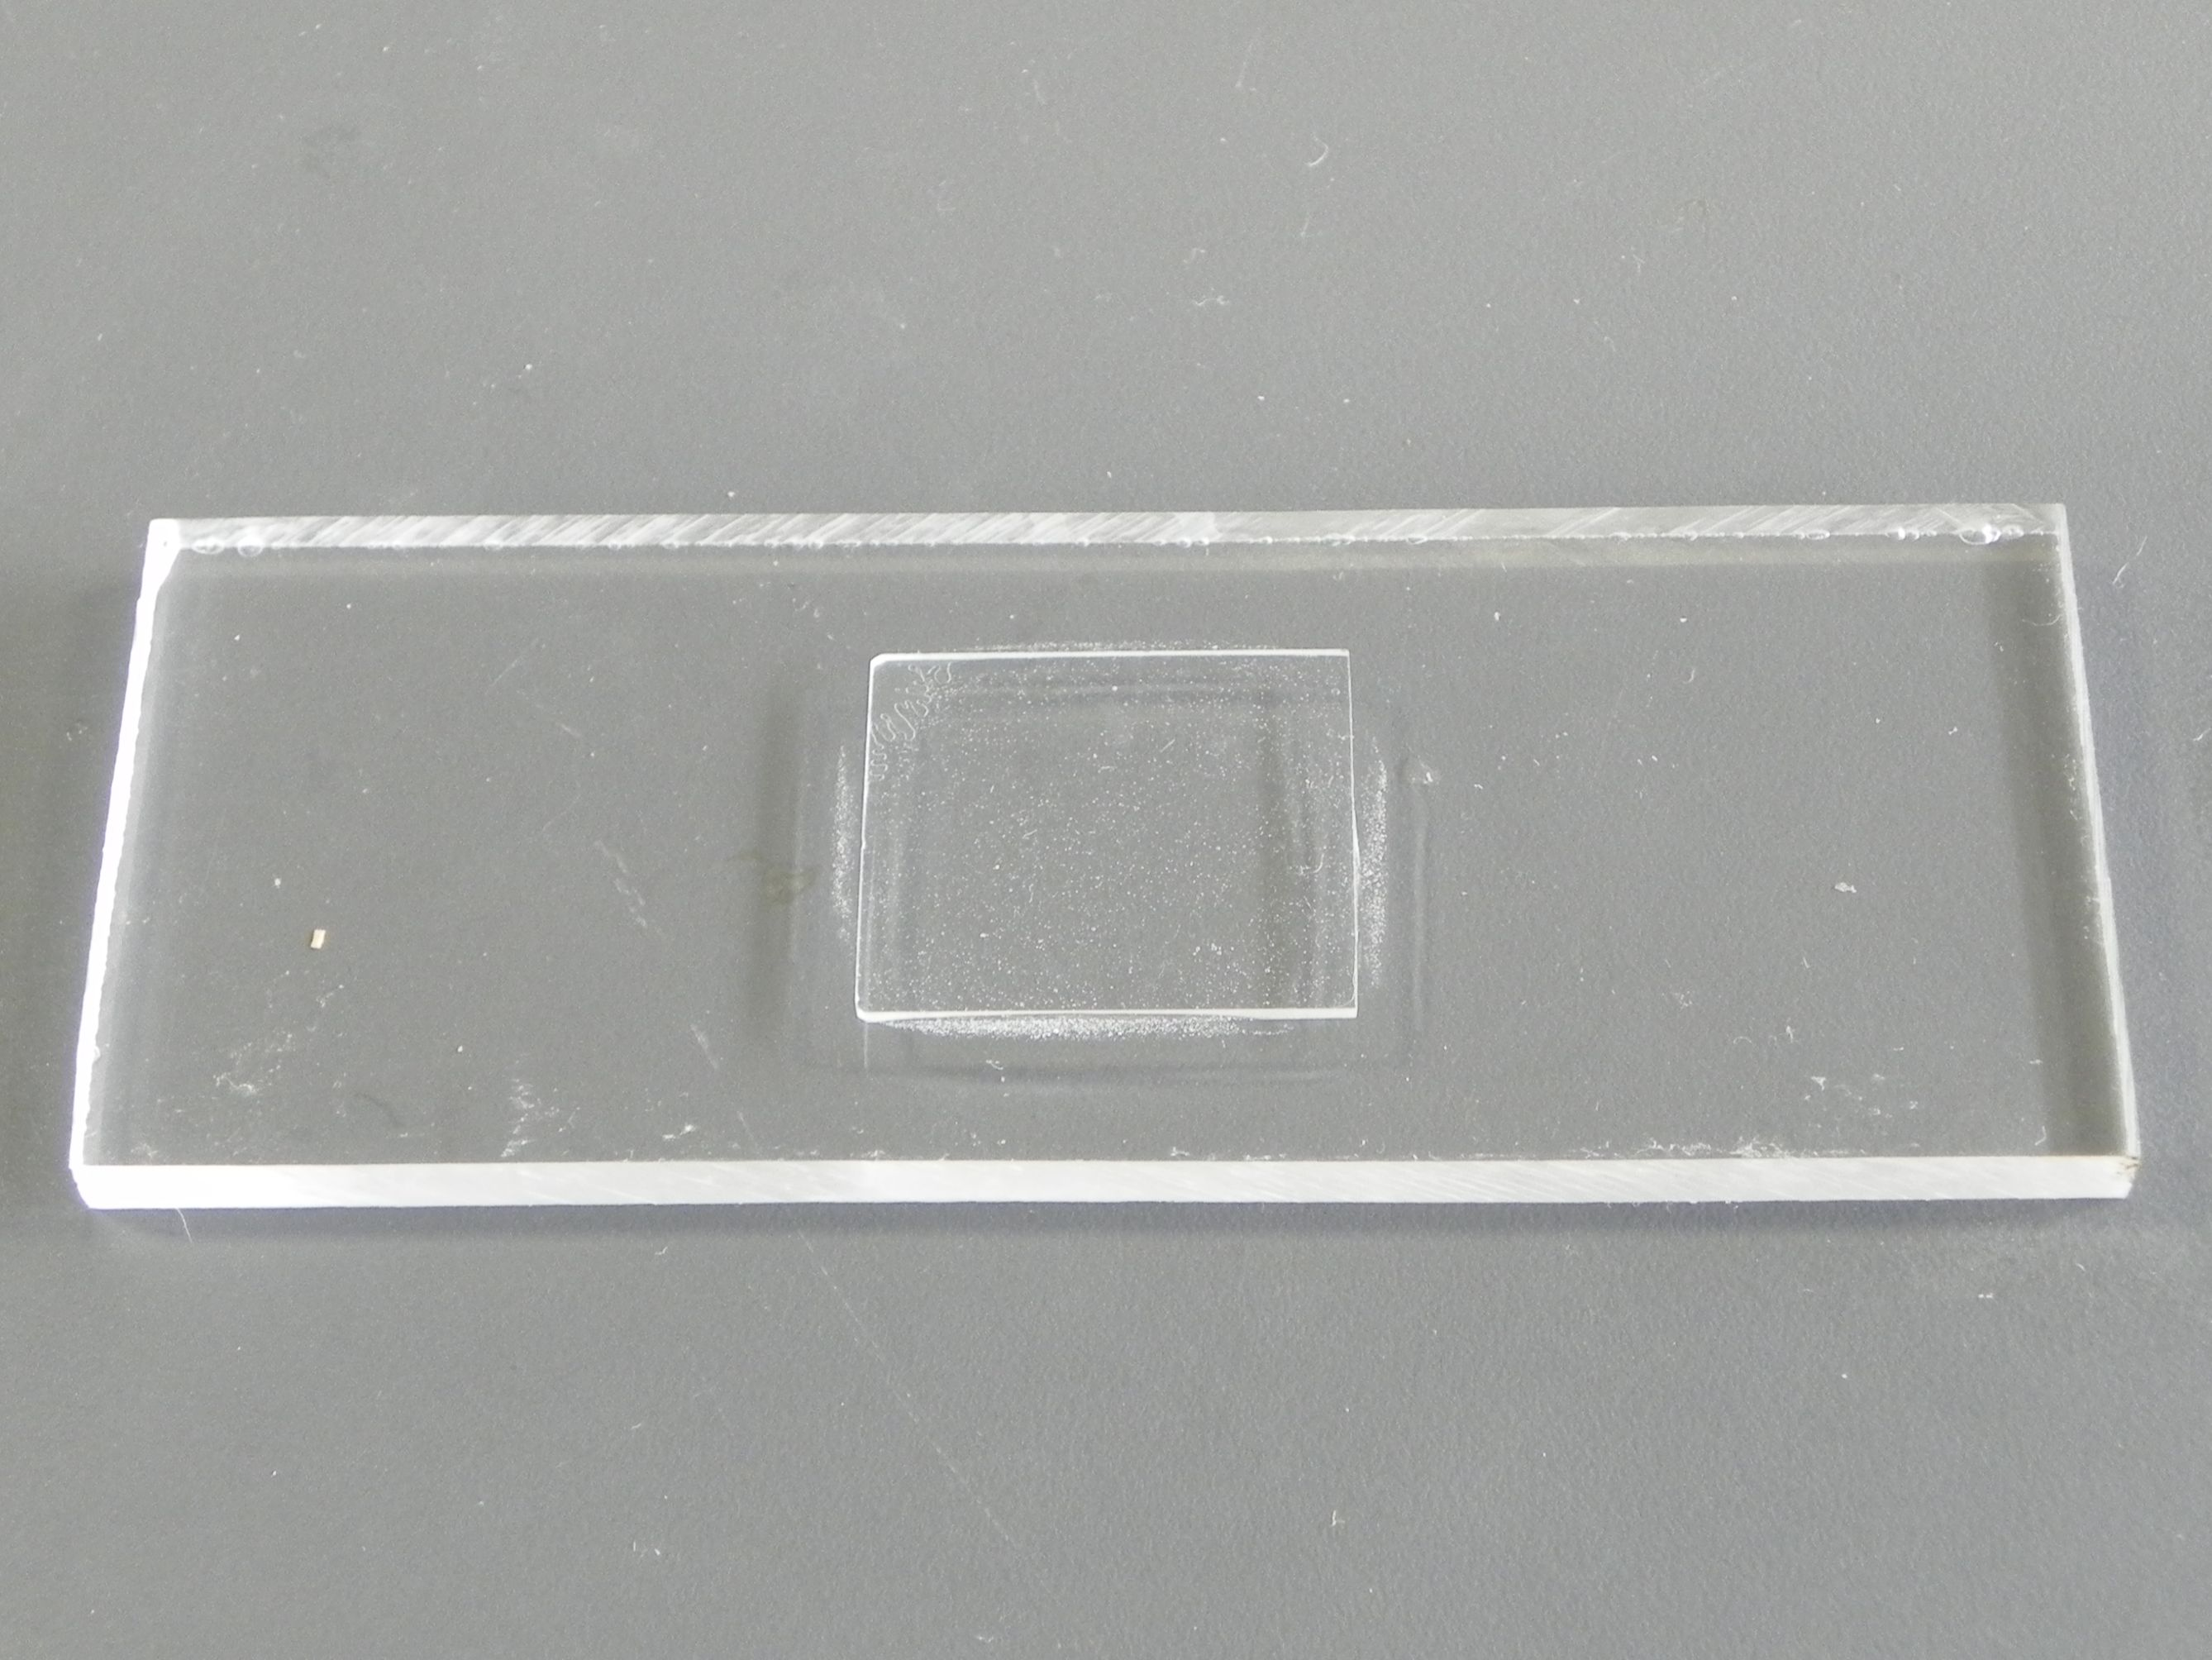
\includegraphics[width=0.5\textwidth]{content/pt1/01-PowerHarvesting/graphics/Photo_streamingPotential_Assembly_Step1.JPG}
      \caption{\label{fig:Photo_streamingPotential_Assembly_Step1}Photo showing half of a glass slide glued to acrylic base plate. Part of the process for constructing a streaming cell.}
    \end{figure}
    \begin{figure}[p]
      \centering
      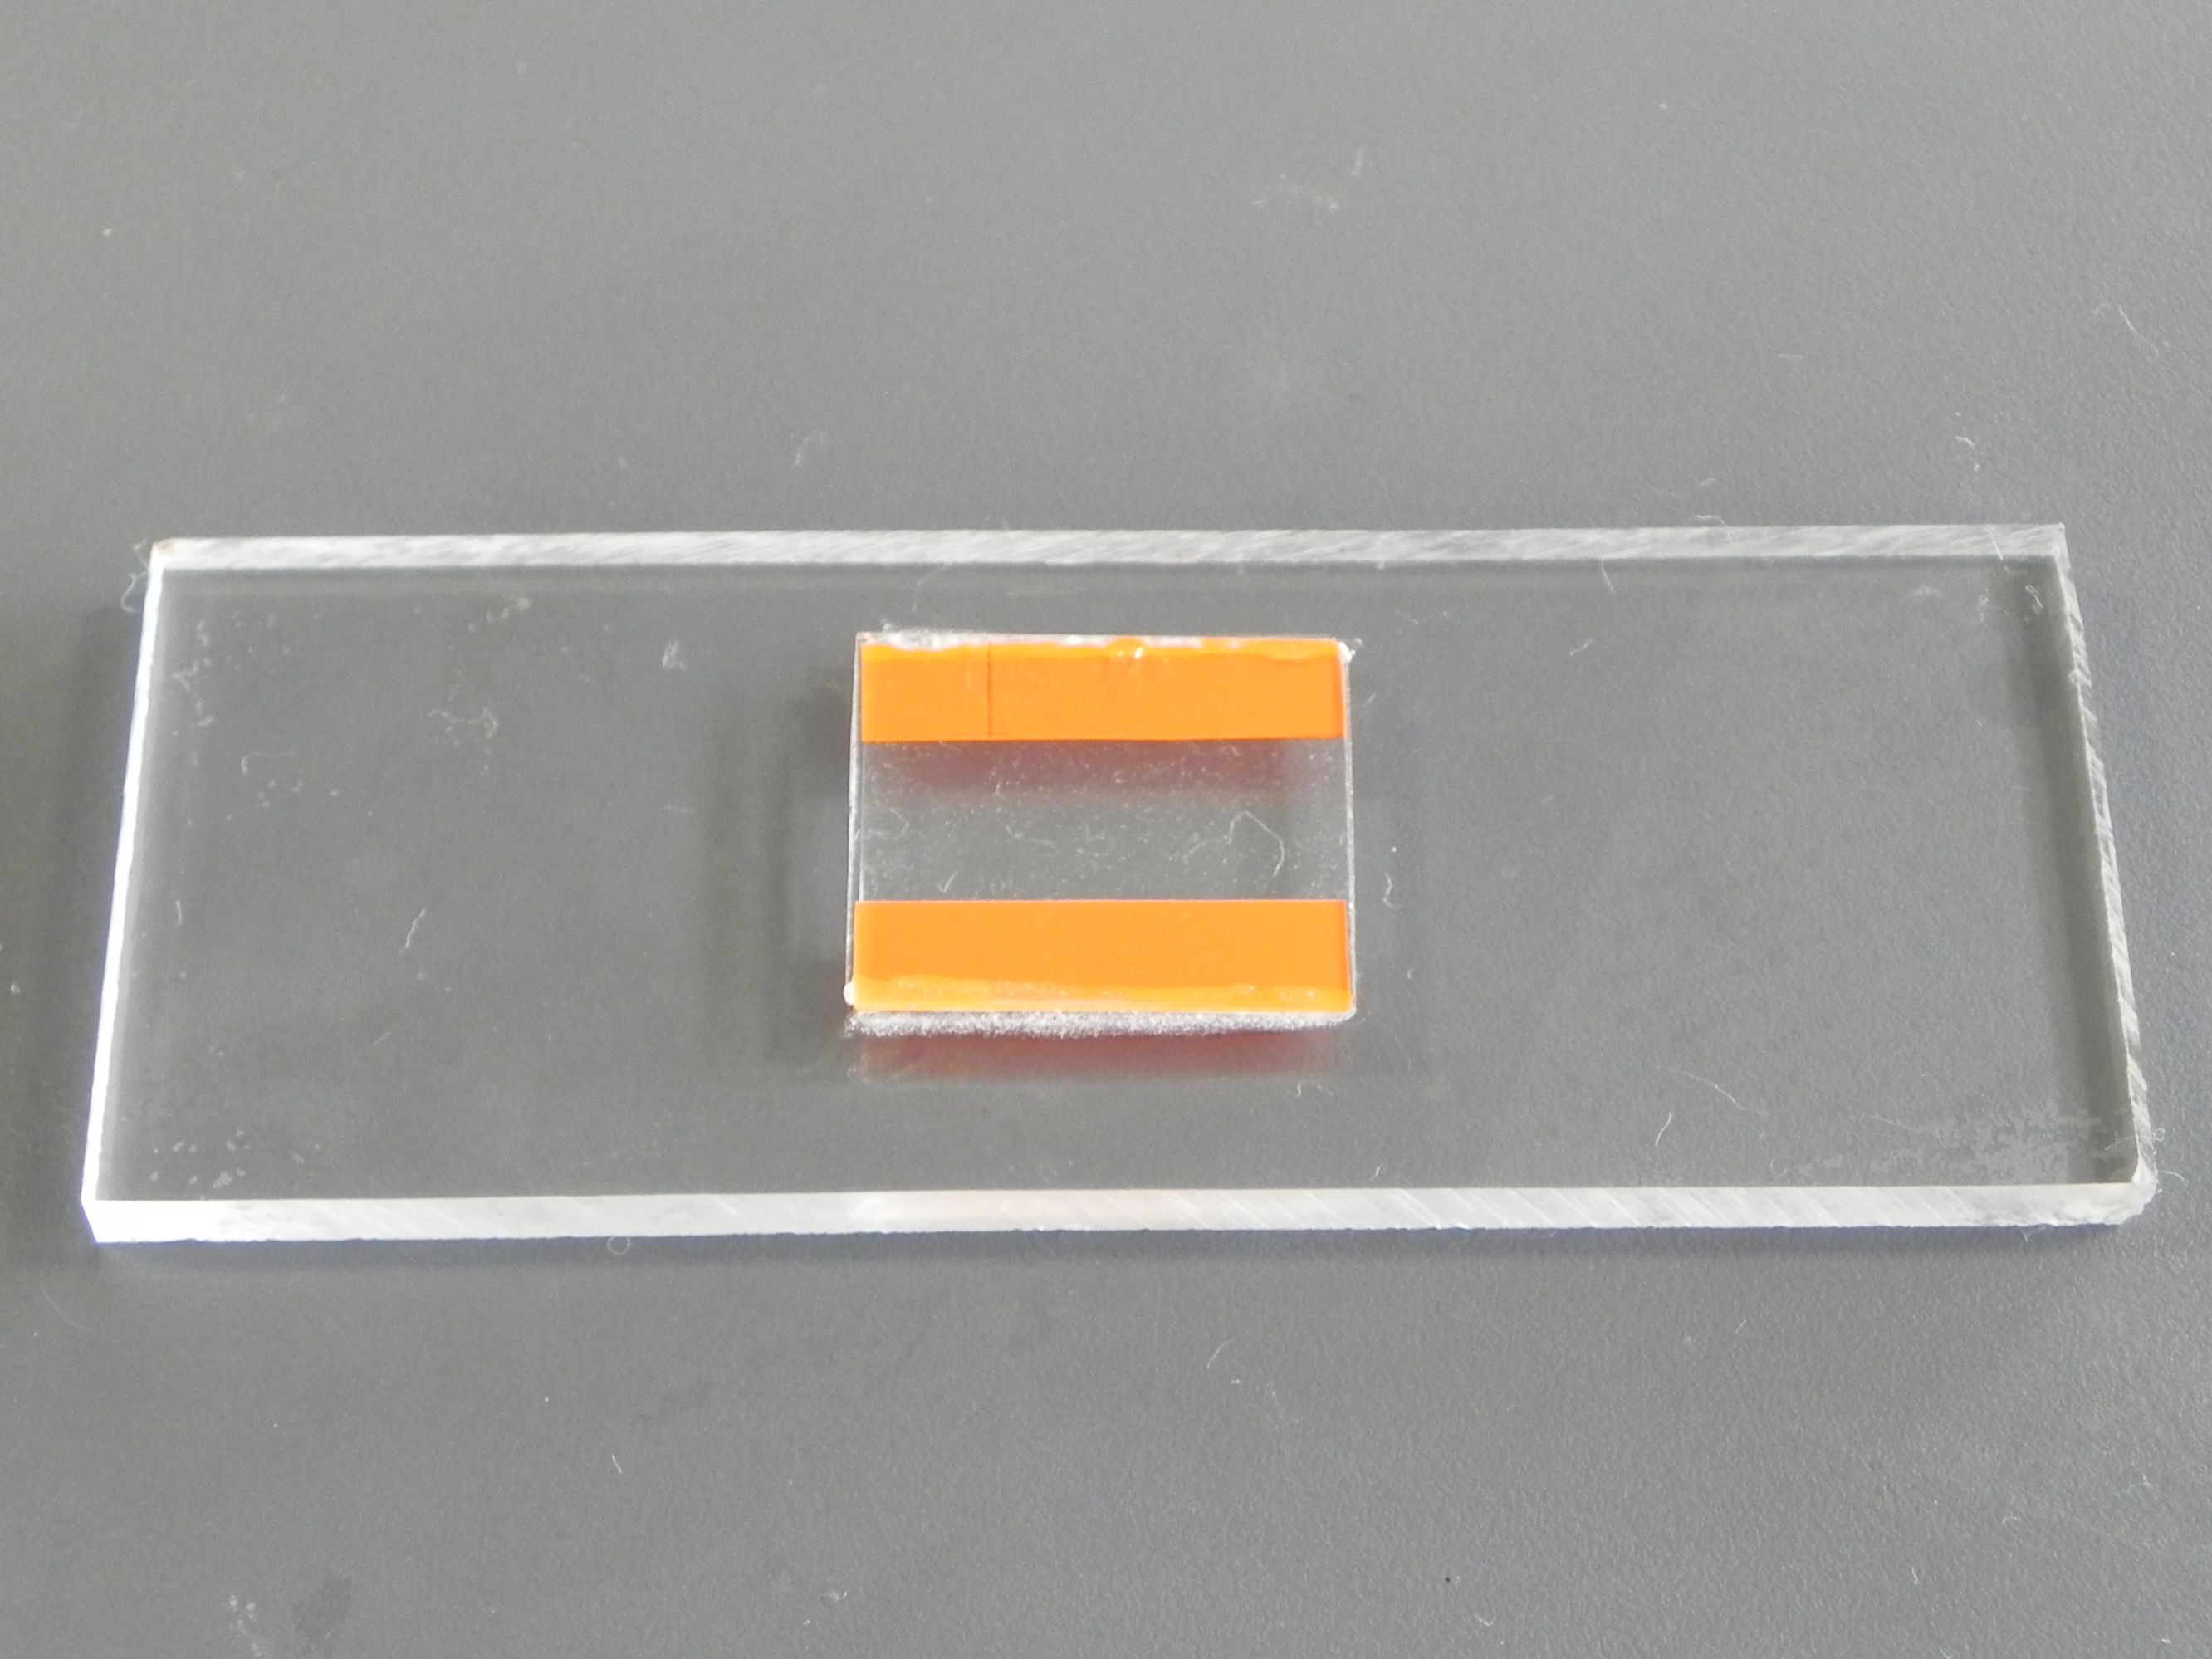
\includegraphics[width=0.5\textwidth]{content/pt1/01-PowerHarvesting/graphics/Photo_streamingPotential_Assembly_Step2.JPG}
      \caption{\label{fig:Photo_streamingPotential_Assembly_Step2}Photo showing plastic shims sandwiched between two slide halves. Part of the process for constructing a streaming cell.}
    \end{figure}
    \begin{figure}[p]
      \centering
      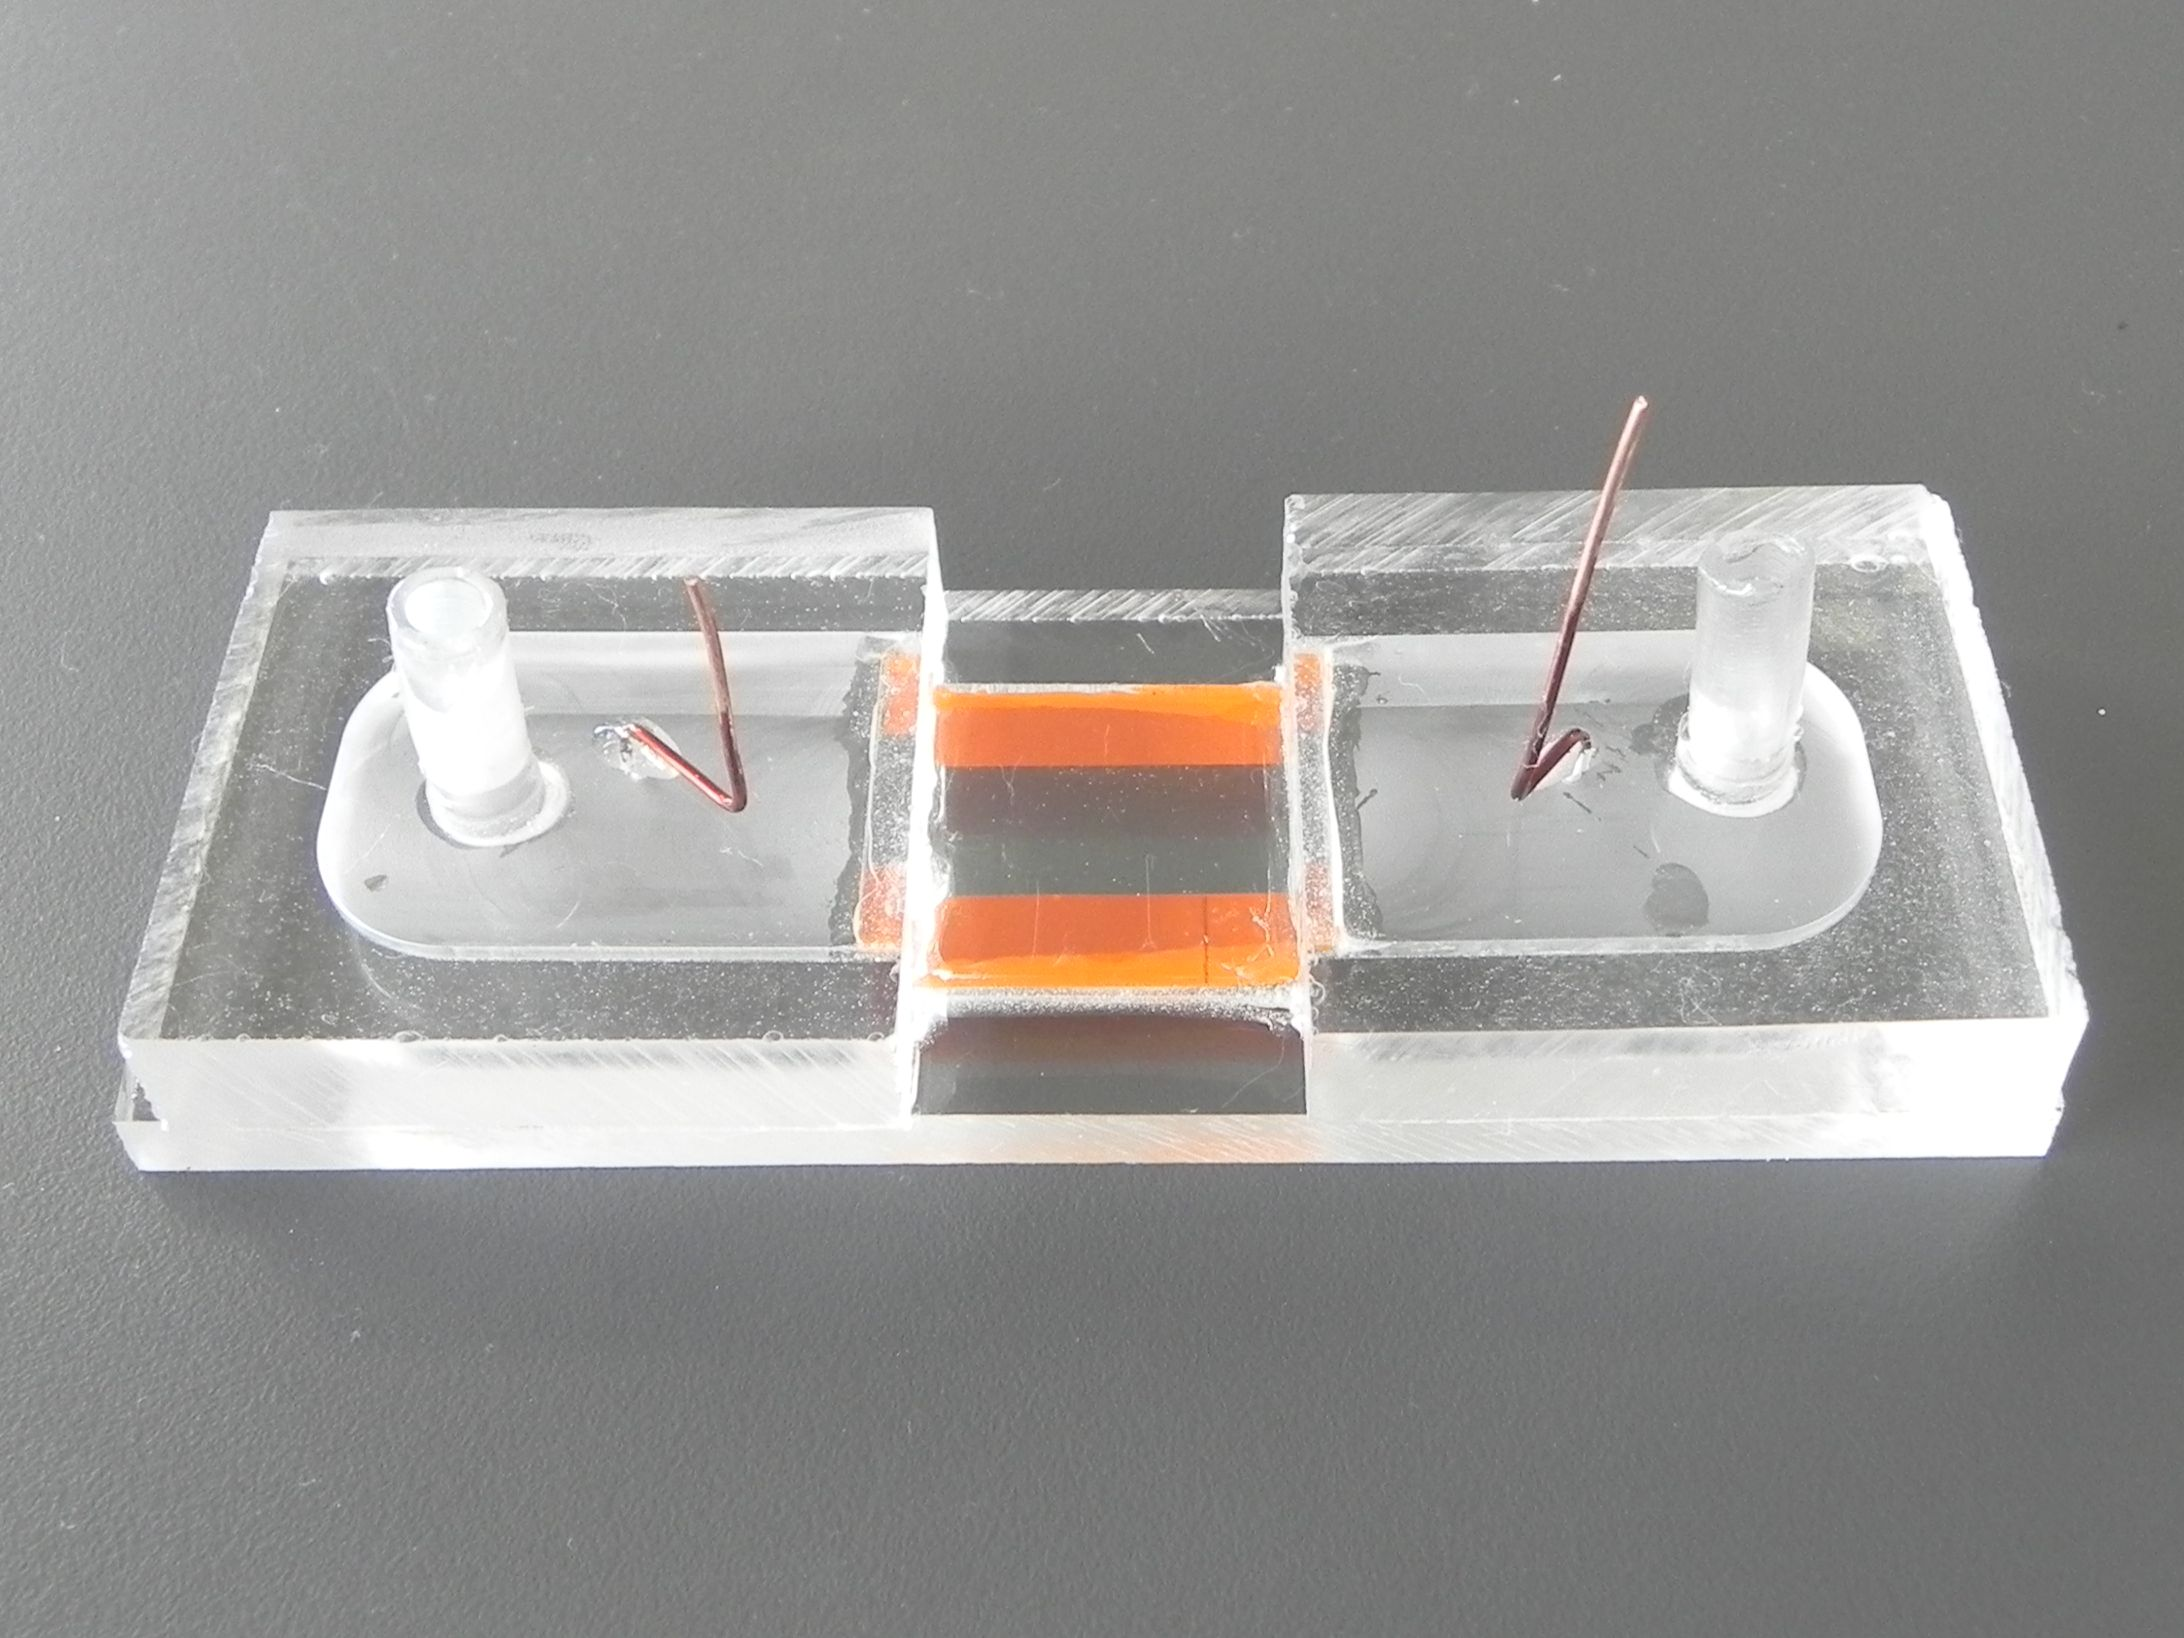
\includegraphics[width=0.5\textwidth]{content/pt1/01-PowerHarvesting/graphics/Photo_streamingPotential_Assembly_Step3.JPG}
      \caption{\label{fig:Photo_streamingPotential_Assembly_Step3}Photo showing final streaming cell assembly.}
    \end{figure}


    \subsubsection*{Construction}

      \begin{table}
        \begin{tabular}{r|c|l}
          Item & Brand & Product details\tabularnewline\hline
          Microscope slides & Sail Brand & JIA 7101WT - 26 x 76mm\tabularnewline
          Shims & Garlock & Colorplast - 50$\,\mu$m,80$\,\mu$m, 120$\,\mu$m and 250$\,\mu$m\tabularnewline
          Epoxy & Selleys & Araldite - Ultra Clear Resin\tabularnewline
          Pressure sensor & Honeywell & 24PC15SMT - 0 -- $\pm$15 PSI\tabularnewline
        \end{tabular}
        \caption{\label{Table_StreamingCell_MaterialsUsed}Materials used to construct the streaming potential cells}
      \end{table}
      Construction began by sectioning standard microscope slides into halves.
      This produced glass panels of approximately \SI{26}{\milli\meter} $\times$ \SI{38}{\milli\meter} $\times$ \SI{1}{\milli\meter}.
      A single panel was then epoxied to an acrylic base plate, as is shown in Figure~\ref{fig:Photo_streamingPotential_Assembly_Step1}.
      Once set, plastic shims were cut to the required size, covered with a very thin layer of epoxy, and placed along the edges of the slide.
      The shims lined the sides of the glass panel such that they left a \SI{1}{\centi\meter} gap through the centre.
      A second glass slide was then placed on top of the shims and epoxy resin used to seal the sides.
      Pressure was applied to the stack while the epoxy set to ensure the epoxy was distributed correctly and to control the channel height.
      A photo of the shims glued between the two slide halves is shown in Figure~\ref{fig:Photo_streamingPotential_Assembly_Step2}.
      Once set, each channel was examined under a microscope to determine the internal channel height.
      Each of the four corners were measured to ensure the internal dimensions remained rectangular once set.
      To finish, acrylic reservoirs where mounted over each end of the channel.
      These reservoirs facilitate the connection of fluid tubes and voltage probes to each end of the channel.
      The final assembly is shown in Figure \ref{fig:Photo_streamingPotential_Assembly_Step3}.
      A full list of materials used to construct the channels is presented as Table~\ref{Table_StreamingCell_MaterialsUsed}.
      A total of ten channels were made and tested using this method.


\section{Measurements}
  \label{sect:part1_energyHarvesting_measuringStreamingCells}


  Of the papers describing experiments using streaming potential cells (\cite{Gu2000,Mala1997,Scales1992,VanderHeyden2006}), I chose that of Gu and Li to replicate~\cite{Gu2000}.
  Their method employs a simple cell design, discussed in the previous section, and a detailed description of the experimental procedure.
  This section details measurement of ten streaming cells based on those of Gu and Li.


  \subsection{Experimental setup}
    \label{sub:part1_energyHarvesting_measuringStreamingCells_experimentalSetup}


    Measurement of each harvester was made in a laboratory using high-sensitivity measurement instruments and a lab water tap.
    Each cell's output power was measured with a precision source measurement unit (SMU) and applied pressure was monitored with a differential pressure sensor.

    The Agilent E5270B is a mainframe system that holds banks of SMUs with connections to a GPIB computer interface.
    The Department of Engineering's E5270 contains three SMUs, each having the ability to measure currents as low as one femto-Ampere.
    The device uses separate `force' and `sense' connections to ensure the voltage/current being set is accurately controlled where they meet.
    Additionally, it uses tri-axial cables to minimise any interference from outside sources, which is important when measuring such low currents.

    The input resistance to the E5270's measurement units are specified as \SI{13}{\giga\ohm}.
    It is essential to use such a high impedance measurement due to the high internal resistance of the cell.
    I later show that the internal electrical resistance of the cell is in the order of \SI{5}{\mega\ohm}, so the E5270's input impedance is roughly two thousand times larger.
    The internal resistance of a typical multimeter is \SI{10}{\mega\ohm}, too close to that of the cell and would therefore affect the measured output.

    The pressure sensor used was a Honeywell 26PC SMT Series differential pressure sensor.
    It came as surface mount package, making it a cost effective solution, but delicate to set up.
    On its exterior are two ports to which rubber tubes are attached.
    Between those ports, internal to the sensor, sits a diaphragm.
    That diaphragm controls the resistance between two nodes in the sensor's bridge circuit (shown in figure \ref{fig:PressureSensorSchematic}).
    \begin{figure}
        \centering
        
\includegraphics{content/pt1/01-PowerHarvesting/graphics/PressureSensorSchematic}
        \caption{\label{fig:PressureSensorSchematic}Schematic diagram of the differential pressure sensor bridge circuit (taken from \cite{Honeywell2003})}
    \end{figure}
    By applying \SI{10}{\volt} DC between the `Vcc' and `GND' pins, the output voltage between outputs `A' and `B' correspond to the applied pressure.
    Measurement of that output voltage was done using the precision measurement mainframe.

    The mainframe was controlled from a PC running Python scripts utilising the open source Python-vxi11 library~\cite{Python-ivi2014}.
    This allows sweeping the amount of current drawn from the harvester while recording the corresponding voltage drop.
    This is the equivalent of varying the load resistance, which allows us to find the point of maximum power transfer.

    \Cref{fig:measurementSetup} shows the measurement setup as a diagram.
    It shows connection of the measurement mainframe, bench-top power supply, streaming cell, pressure sensor, and the lab tap.
    Table~\ref{tab:measurementSetup_legend} provides details of the abbreviated electrical connection labels used in the figure~\ref{fig:measurementSetup}.

    \begin{figure}
        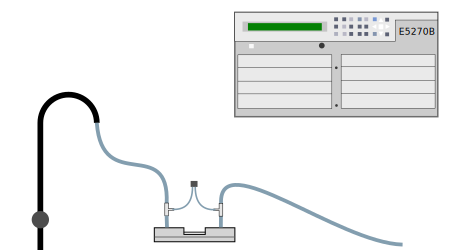
\includegraphics{content/pt1/01-PowerHarvesting/graphics/measurementSetup}
        \caption{\label{fig:measurementSetup}Diagram showing the measurement setup used to measure power output from streaming cell energy harvesters.}
    \end{figure}

    \begin{table}
        \centering
        \begin{tabular}{r|l}
        CELL - A & Voltage/current at high-pressure side of cell\\
        PRESS. - A & Output A of pressure sensor\\
        PRESS. - B & Output B of pressure sensor\\
        CELL - B & Voltage/current at low-pressure side of cell
        \end{tabular}
        \caption{\label{tab:measurementSetup_legend}Definitions for labels used in \cref{fig:measurementSetup}}
    \end{table}


  \subsection{Measurement issues}


    There were two issues with the measurement setup that may have impacted  measurements.
    Firstly, the electrodes used were copper and are susceptible to polarisation by electrolysis.
    Secondly, the differential pressure sensor was only rated to 15\thinspace PSI (approximately \SI{100}{\kilo\pascal}), less than half the maximum pressure developed across the cell.

    Electrolysis on at the electrode surface would cause the electrodes to polarise, resulting in a semi-permanent offset voltage appearing between electrodes.
    That offset voltage would be opposite in polarity to what is developed while cell was in operation.
    By reversing the flow of water through the cell, the polarisation should be reversed.
    The use of more suitable electrode materials would reduce this effect, for instance platinum black electrodes.
    Copper was used for the electrodes as it was cheap, easily obtainable, and easy to work with.
    Offset voltages can be removed after measurement by subtraction.
    This was not a perfect solution, but the offset voltage could be measured and accounted for so was left as-is.

    From measurement of the output \emph{voltage} of the cells, the presented graphs and figures have been adjusted to remove the effects of electrolysis.
    This was done by adding an offset to the measured data to shift the y-intercept up to \SI{0}{\volt}.
    This represents the situation where platinum black electrodes been used.
    As no absolute data is taken from these measurements, the y-intercept adjustment does not affect any subsequent predictions made about the cells.
    Only the gradient of the output relative to the pressure applied is used, and even then, only to select a suitable candidate cell for power measurement.
    \emph{Most importantly}, no offsets have been applied to measurements of the cell power output.

    Although the maximum rated pressure of sensor was 15\thinspace PSI (approximately \SI{100}{\kilo\pascal}), the sensor's output remained linear up to our maximum pressure of 40\thinspace PSI (\SI{275}{\kilo\pascal}).
    I expect that exceeding the sensors specified pressure will result in a lower `mean time to failure', but its output remained true.
    As a precaution, a tyre pressure gauge was used to roughly confirm the output of the sensor at the end of the cell measurements.
    This was a crude test, however its output matched that of the differential pressure sensor so was taken as an indication of accuracy.


\section{Results}
  \label{sect:part1_energyHarvesting_results}


  Results from streaming cell measurement are broken into two sub-sections.
  The first presents the output voltage of the ten cells in response to applied water pressure.
  From these measurements, the cell with the highest voltage/pressure ratio is found.
  The second sub-section shows the maximum power that can be harvested from that cell.
  These are the most important measurements as they reveal the energy conversion efficiency of the cells.


  \subsection{Streaming voltage versus pressure}



    \Cref{fig:streamingCell_all_adjusted} shows adjusted results of streaming voltage measurements from each of the ten cells.
    A full set of figures, one cell per graph, can be found in \cref{appendix:streamingCellMeasurements} as \crefrange{fig:VvsP_26um}{fig:VvsP_245um}.
    It represents the first successful measurements I had made of streaming cells.
    During these measurements three cells burst under pressure, two were dropped and subsequently shattered, and one suffered epoxy failure.
    No measurements of flow rate or output current were made during these early experiments.
    As a result they reveal very little about the efficiency of the cells themselves.
    We cannot determine either the mechanical energy put into the cells, nor the output power available.
    However, we can relate these measurements to those made by Gu and Li as will be shown and discussed shortly.

    \begin{figure}
        \centering
        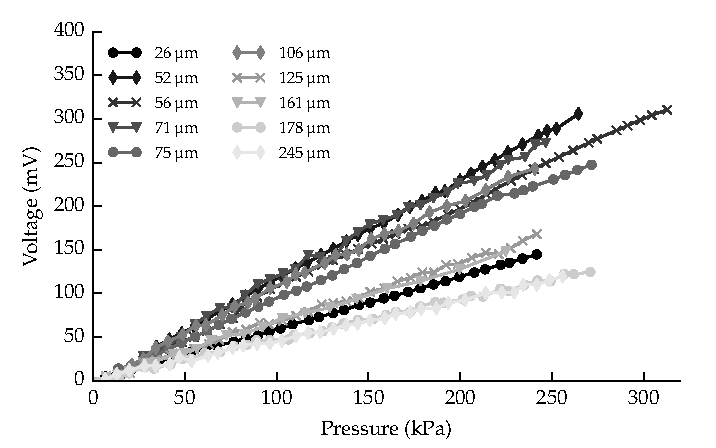
\includegraphics{content/pt1/01-PowerHarvesting/graphics/graph_streamingVoltageGradient_vs_height}
        \caption{\label{fig:streamingCell_all_adjusted}Plot showing adjusted streaming voltages versus applied pressure.}
    \end{figure}

    \begin{figure}
        \centering
        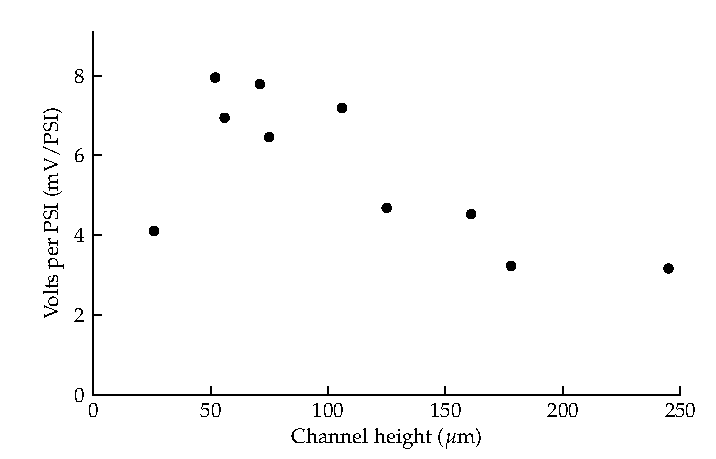
\includegraphics{content/pt1/01-PowerHarvesting/graphics/streamingCell_slopeVsChannelHeight}
        \caption{\label{fig:streamingCell_scatter_voltGradVsHeight}Scatter plot of voltage/pressure gradient versus channel height for each of the measured channels.}
    \end{figure}

    \begin{figure}
        \centering
        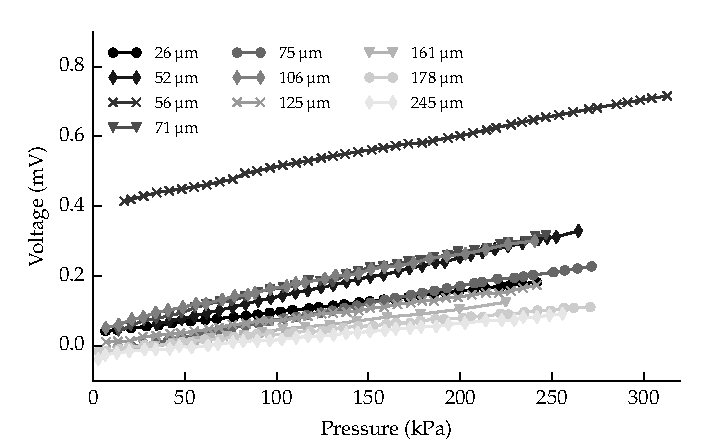
\includegraphics{content/pt1/01-PowerHarvesting/graphics/graph_streamingVoltageGradient_vs_height_noCorrection}
        \caption{\label{fig:streamingCell_all_unadjusted}Plot showing unadjusted streaming voltages versus applied pressure.}
    \end{figure}

    The cell having an internal height of \SI{56}{\micro\meter} required an offset adjustment of \SI{405}{\milli\volt} to remove its vertical offset.
    This indicates that the electrodes were highly polarised by the time measurements were made.
    This effect is especially evident in \cref{fig:streamingCell_all_unadjusted}, which shows raw measured data without vertical offset adjustment.
    Some of the traces exhibit a certain amount of `jitter' in their pressure-to-voltage gradients.
    This is likely due to the time difference between adjacent measurement points.
    Measurement points were not taken monotonically, instead being extracted from a number of pressure cycles.

    \Cref{fig:streamingCell_scatter_voltGradVsHeight} shows the streaming voltage to pressure gradients versus channel height.
    This data has been taken from the previous graph (\cref{fig:streamingCell_all_adjusted})) to show the response as a function of channel height.

    % Edit checkpoint 2015-09-13 19:43


  \subsection{Output power versus load resistance}


    \begin{figure}
        \centering
        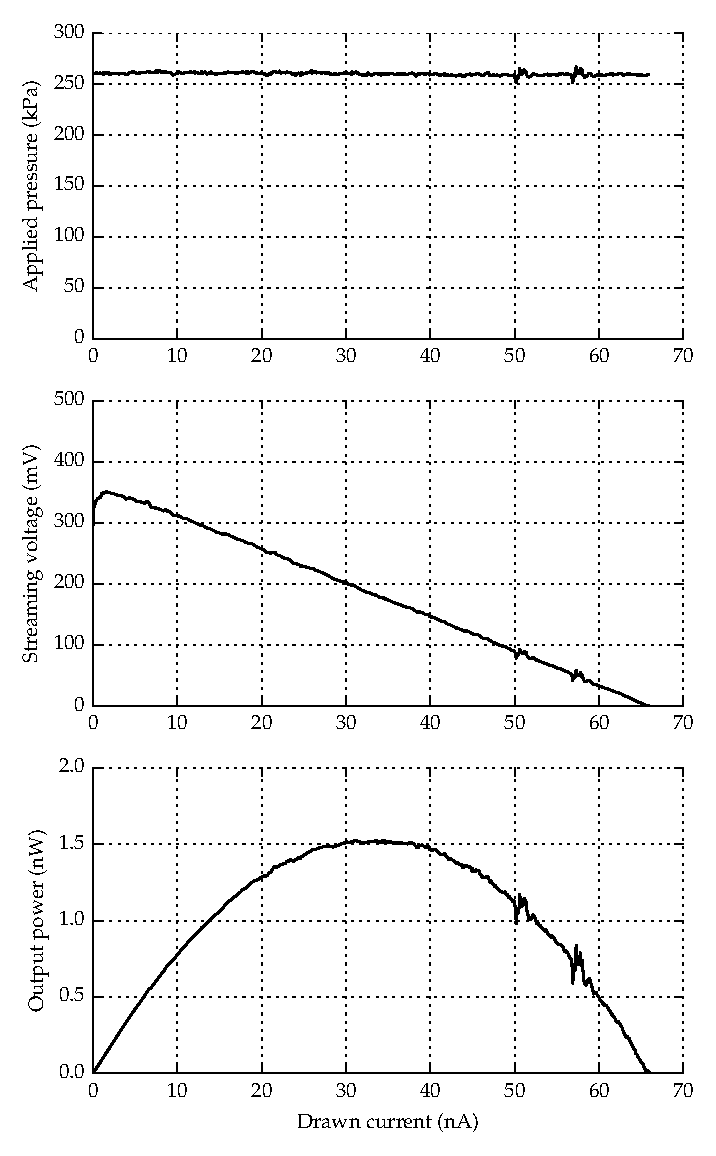
\includegraphics{content/pt1/01-PowerHarvesting/graphics/graph_streamingCell_outputPower_resistanceSweep}
        \caption{\label{fig:streamingCell_maxPower}Graph showing output power versus effective load resistance for a \SI{71}{\micro\metre} high channel at a pressure of \SI{260}{\kilo\pascal}.}
    \end{figure}

    \Cref{fig:streamingCell_maxPower} shows the characteristic power curve of the \SI{71}{\micro\meter} high streaming cell channel.
    Pressure fluctuations near the end of the experiment are due to usage of the departments water system.
    Their effect is visible in both the streaming voltage and output power traces, highlighting the strong coupling to applied pressure.

    The maximum power delivered by the cell was \SI{1.52}{\nano\watt}, corresponding to a current draw of \SI{33.5}{\nano\ampere} with a streaming voltage of \SI{182}{\milli\volt}.
    Generating this power required \SI{260}{\kilo\pascal} of pressure, resulting in a flow rate of \SI{2.05}{\milli\litre\per\second}.
    % This equates to \SI{539}{\milli\watt} of pumping power lost to the device and therefore an energy conversion efficiency of \SI{0.28}{\micro\percent}.
    This equates to \SI{539}{\milli\watt} of pumping power lost to the device and therefore an energy conversion efficiency of \SI{2.8e-9}.


\section{Discussion}
  \label{sect:part1_energyHarvesting_discussion}


  Initial measurements of streaming voltage revealed that the output voltage is directly proportional to applied pressure.
  Containing pressures reaching \SI{260}{\kilo\pascal} within glass structures is difficult.

  Comparing the streaming voltage measurements taken from each of the ten cells to the measurements made by Gu and Li yielded surprising results.
  In their paper~\cite{Gu2000}, they determined the zeta potential ($\zeta$) and surface conductivity ($\lambda$) by plotting measurements and fitting a linear equation to their data.
  The use the y-intercept of the resulting line to give the inverse zeta potential and the slope of the line gave information about the surface conductivity.

  \begin{figure}
      \centering
      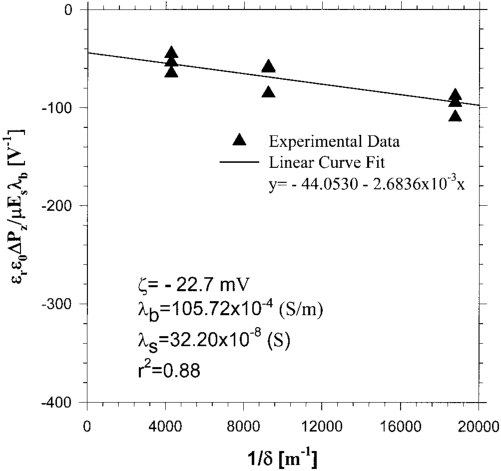
\includegraphics{content/pt1/01-PowerHarvesting/graphics/GuLi_DIUF}
      \caption{\label{fig:Gu_Li_comparison_DUIF}Plot showing measured data from Gu and Li's paper on streaming cells relating the streaming voltage and pressure differential to the channel height with distilled water as the working fluid~\cite{Gu2000}.}
  \end{figure}

  \begin{figure}
      \centering
      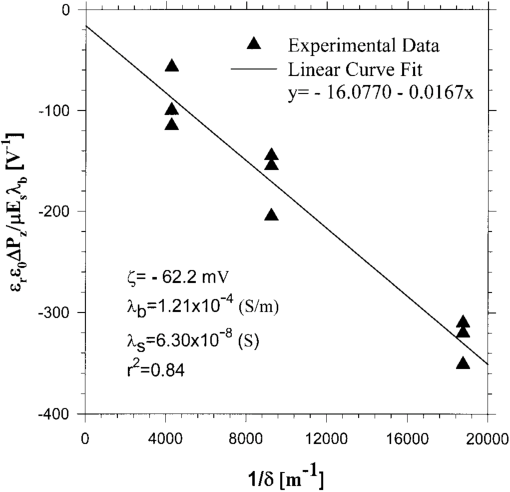
\includegraphics{content/pt1/01-PowerHarvesting/graphics/GuLi_NaCl}
      \caption{\label{fig:Gu_Li_comparison_NaCl}Plot showing measured data from Gu and Li's paper on streaming cells relating the streaming voltage and pressure differential to the channel height with a \SI{1}{\milli\mole} sodium chloride solution as the working fluid~\cite{Gu2000}.}
  \end{figure}

  Their results for three streaming cells are shown here (taken from \cite{Gu2000}) as \cref{fig:Gu_Li_comparison_DUIF,fig:Gu_Li_comparison_NaCl}.
  The first (\cref{fig:Gu_Li_comparison_DUIF}) shows measurements when distilled water is used as the working fluid, the second (\cref{fig:Gu_Li_comparison_NaCl}) shows the measurements for a weak saline solution.
  It is interesting to note that they have what looks to be fairly linear data, although it is hard to tell with only three channel sizes.

  \begin{figure}
      \centering
      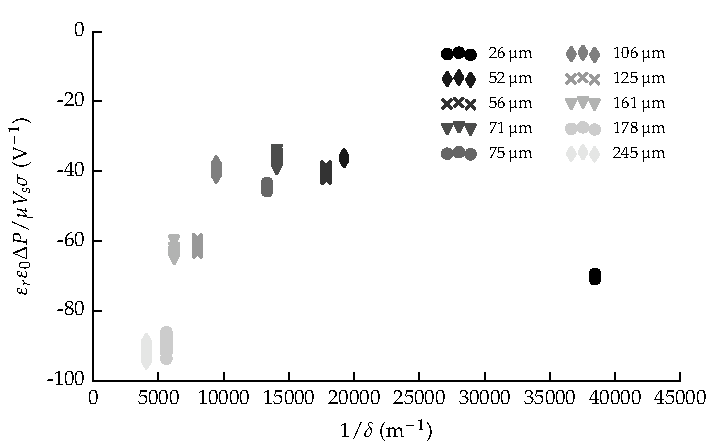
\includegraphics{content/pt1/01-PowerHarvesting/graphics/graph_streamingComparison_gu}
      \caption{\label{fig:streamingCell_scatter_Gu_Li}Scatter plot with results of streaming cell measurements in terms of those made by Gu and Li~\cite{Gu2000} (for comparison).}
  \end{figure}

  By comparison, \cref{fig:streamingCell_scatter_Gu_Li} plots the same variables from measurements taken from the ten streaming cells fabricated here.
  In this graph, the following substitutions have been made: $\lambda_{b}$ has been replaced with $\sigma$ (both refer to the bulk conductivity of the solution), and $E_{s}$ has been replaced with $V_{s}$, (both refer to the streaming potential).
  The response to variation of channel height is clearly non-linear.
  Their method of finding the zeta potential rests on the following rearrangement:
  \begin{eqnarray}
      \frac{\varepsilon_{r}\varepsilon_{0}\Delta P}{\mu V_{s}\sigma} = \frac{1}{\zeta} + \left( \frac{2\,\lambda}{\zeta \sigma}\right)\,\frac{1}{\delta}
  \end{eqnarray}
  where $\lambda$ is the surface conductivity and $\delta$ is the channel height.
  So as the channel height ($\delta$) tends to infinity, the left hand side tends toward the zeta potential ($\zeta$).
  This notion seems counter intuitive since the zeta potential is defined at the plane of shear (as shown in \cref{fig:doubleLayer_anatomy}), relative to the solution bulk.
  The equation is stating that no-matter how far you separate the walls, the minimum voltage-pressure gradient you can get is still set by the zeta potential.

  Measurement of the output power generated by the \SI{71}{\micro\meter} streaming cell is promising.
  From this measurement the power transfer curve is evident.
  Referring back to the model presented as \cref{fig:StreamingCell_Schematic-representation}, we can now calculate the channels internal electrical resistance ($R_{cell}$).
  We know from the graph that the maximum power transfer occurred at a current of \SI{33.5}{\nano\ampere} with a streaming voltage of \SI{182}{\milli\volt}.
  Via Ohm's law this equates to a load resistance ($R_{out}$) of \SI{5.43}{\mega\ohm}, which from the maximum power theorem we know must be equal to the cells internal resistance.


\section{Concluding Remarks}
  \label{sect:part1_energyHarvesting_conclusion}

  Conversion of mechanical pumping into electrical energy can be done with narrowly separated plates of glass.
  The conversion efficiency seen here was low, much lower than reported in the literature.
  A channel \SI{1}{\centi\meter} by \SI{3}{\centi\meter} by \SI{71}{\micro\meter} produced \SI{1.5}{\nano\watt} under a pressure differential of \SI{260}{\kilo\pascal}.
  % That took \SI{359}{\milli\watt} of pumping power to produce, yielding an efficiency in the order of \SI{0.1}{\micro\percent}.
  That took \SI{359}{\milli\watt} of pumping power to produce, yielding an efficiency in the order of \SI{1e-9}.
  Precision engineering, with regards to cell construction, will likely lead to greater efficiency.
  This is based on reports from the literature, where higher efficiency channels utilised much narrower channels.

  Measurements of ten streaming cells were compared to the results published by Gu and Li.
  The linear relationship of Gu and Li between channel height and their plotted parameter could not be reproduced.
  Instead, results showed a highly non-linear relationship as shown in~\cref{fig:streamingCell_scatter_Gu_Li}.
  The gradient of measurement points within the range of channel heights measured by Gu and Li is reversed.
  The reason for the discrepancy is not clear.

  The streaming voltage was found to scale linearly with the applied pressure.
  This could potentially be useful as a means of sensing water flow rates.
  A dual purpose such as power sourcing and flow measurement lends itself well to water metering applications.


  % Edit checkpoint 2015-09-13 19:49
